\chapter{Εισαγωγή}

\noindent Οι τεχνολογικές εξελίξεις, που παρατηρούνται τα τελευταία έτη, έχουν 
οδηγήσει στην ευρεία διάθεση παλαιοτέρα απρόσιτων προϊόντων. Συγκεκριμένο 
παράδειγμα αποτελεί η τεχνολογία των εναέριων ρομποτικών συστημάτων και, 
ειδικότερα, των μη-επανδρωμένων αεροχημάτων (ΜΕΑ), η οποία συνιστούσε προνόμιο 
των πολεμικών βιομηχανιών μέχρι πριν μερικά χρόνια. Πλέον, αποτελεί μία από τις
πιο έντονα αναπτυσσόμενες αγορές παγκοσμίως, με συνεχώς εντονότερο ενδιαφέρον 
και από τους ακαδημαϊκούς χώρους. 

Το ενδιαφέρον αυτό, δικαιολογείται από την πληθώρα εφαρμογών, που μπορούν να 
ικανοποιήσουν τα ΜΕΑ, εφαρμογές όπως χαρτογράφηση και αεροβιντεοσκόπηση, 
περιβαλλοντικές και κλιματικές μετρήσεις, αποστολές ανθρωπιστικού χαρακτήρα,
γεωργία ακριβείας καθώς και εφαρμογές ασφάλειας και παρακολούθησης.

Τα ΜΕΑ συναντώνται σε διάφορες διατάξεις, με κύριες τα πολυκόπτερα 
\tl{(Multicopters)}, τα σταθερής πτέρυγας \tl{(Fixed-Wing)} και τα υβριδικά. Τα 
πολυκόπτερα αεροχήματα δίνουν την δυνατότητα κίνησης μεγάλης ακρίβειας, καθώς 
και την δυνατότητα εκτέλεσης πολύπλοκων ελιγμών. Υστερούν, ωστόσο, σε οικονομική 
κατανάλωση, με αποτέλεσμα την μειωμένη αυτονομία. Τα ΜΕΑ σταθερής πτέρυγας, 
εκμεταλλευόμενα τον αεροδυναμικό τους σχεδιασμό, επιτυγχάνουν μικρή κατανάλωση 
ενέργειας και συνεπώς μεγάλη αυτονομία. Ωστόσο, παρουσιάζουν μειωμένες 
δυνατότητες σε ελιγμούς σε σύγκριση με τα πολυκόπτερα. Τέλος τα υβριδικά 
συνδυάζουν τα χαρακτηριστικά των δύο παραπάνω διατάξεων, επιτυγχάνοντας 
μεγάλους χρόνους πτήσης και σημαντική ευελιξία.

Η παρούσα διπλωματική εργασία εκπονήθηκε στα πλαίσια του ερευνητικού 
προγράμματος \tl{"}Αυτόνομο φορητό σύστημα μη-επανδρωμένου αεροχήματος πολλαπλών 
ρόλων, \tl{MULTIROLE PORTABLE UAS "MPU"}\tl{"}. Το συγκεκριμένο ερευνητικό 
πρόγραμμα έχει ως στόχο την μελέτη και κατασκευή ενός μη-επανδρωμένου 
αεροχήματος, υβριδικής διάταξης \tl{VTOL} \tl{(Vertical Takeoff and Landing)}, 
το οποίο εκτελεί την κύρια πτήση του ως αερόχημα σταθερής πτέρυγας, ενώ 
λειτουργεί ως τρικόπτερο για τις διαδικασίες προσγείωσης και απογείωσης.

\begin{figure}[H]
    \centering
    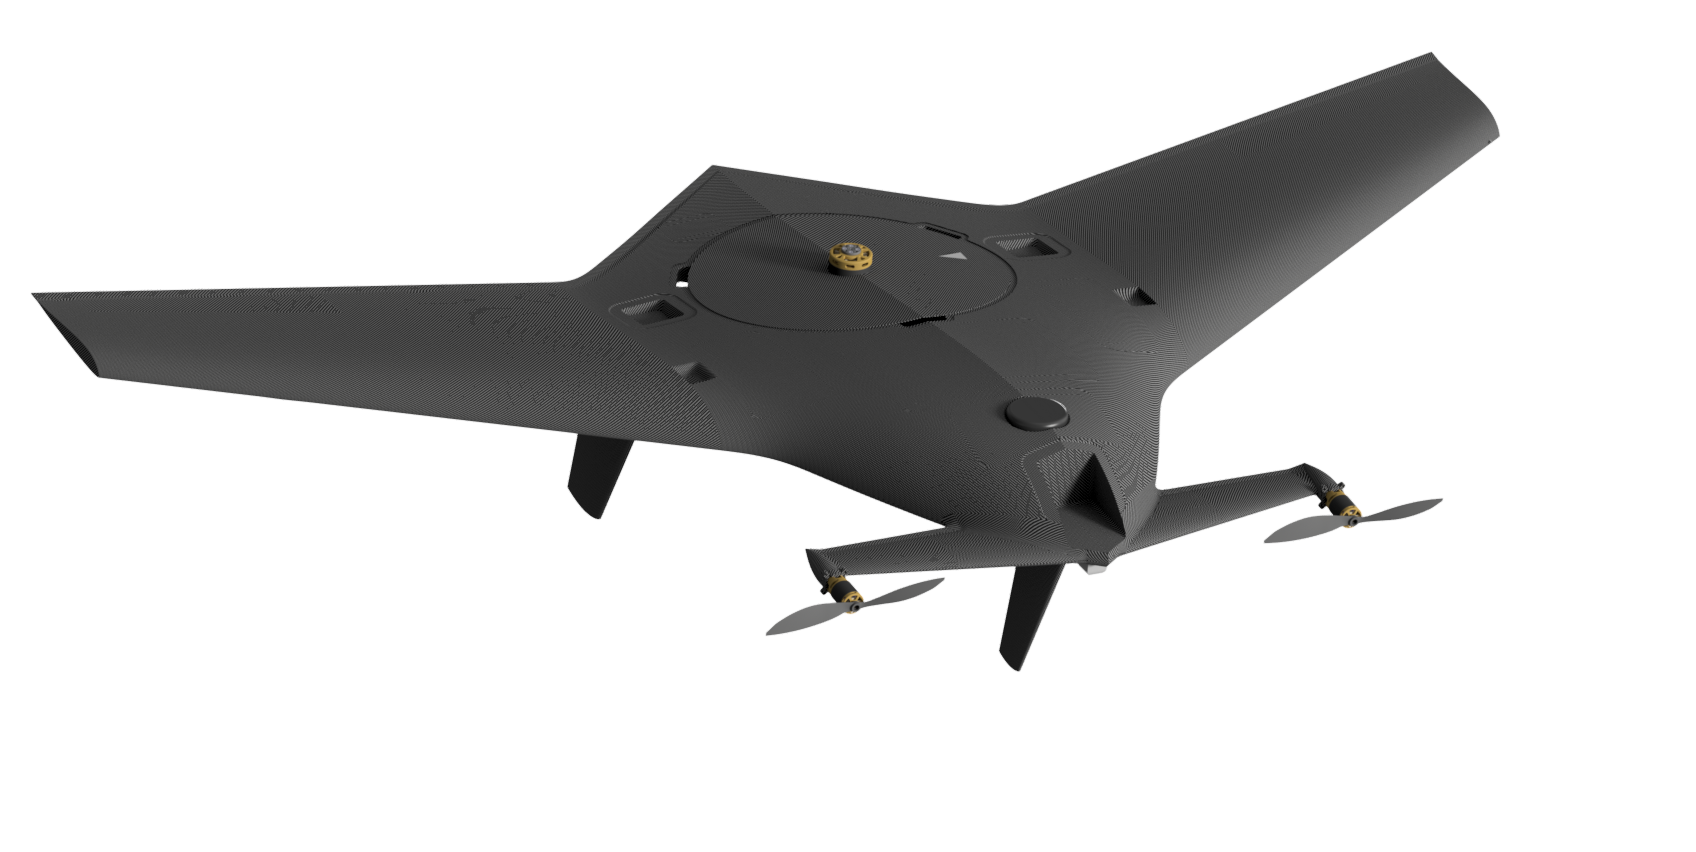
\includegraphics[width=0.8\textwidth]{Skoupa/RX-4_Assembly_Positioning_v6.png}
    \caption{Αυτόνομο φορητό σύστημα μη-επανδρωμένου αεροχήματος πολλαπλών 
    ρόλων, (\tl{MPU})}
\end{figure}

\subsection{Διατύπωση Προβλήματος και Στόχοι}

\noindent Ο στόχος της παρούσας διπλωματικής είναι ο σχεδιασμός και η υλοποίηση 
ενός συστήματος ελέγχου, για την αυτόματη καθοδήγηση του προαναφερόμενου 
αεροχήματος, σε μία προδιαγεγραμμένη τροχιά, με επιθυμητή ευστάθεια και 
σθεναρότητα, για την αιώρηση του ως τρικόπτερο.

\noindent Για την επίτευξη των παραπάνω στόχων, ακολουθείται η εξής διαδικασία
\begin{itemize}
    \item Κινηματική και κινητική ανάλυση του τρικοπτέρου στο χώρο για την 
    μοντελοποίηση της δυναμικής του συμπεριφοράς.
    \item Ανάπτυξη και εφαρμογή ενός συστήματος μη-γραμμικού ελέγχου για την 
    ικανοποίηση των στόχων.
    \item Σχεδιασμός και κατασκευή πειραματικής διάταξης.
    \item Πειραματική εφαρμογή και ανάλυση των αποτελεσμάτων.
\end{itemize}

\subsection{Βιβλιογραφική Ανασκόπηση}

\noindentΤο τρικόπτερο, που εξετάζεται σε αυτήν την εργασία, είναι εξοπλισμένο 
στους δύο από τους τρεις κινητήρες, με μηχανισμό, ο οποίος επιτρέπει την 
περιστροφή του συστήματος έλικα-κινητήρας ως προς το κύριο σώμα του αεροχήματος.
Συνήθως, επιλέγεται άρτιος αριθμός ελίκων, με σκοπό την αλληλοαναίρεση των 
αναπτυσσόμενων ροπών αντίδρασης. Στην περίπτωση μας, λόγω περιττού αριθμού 
ελίκων, οι μηχανισμοί περιστροφής επιτυγχάνουν την εξάλειψη εναπομεινάντων 
ροπών. Η συγκεκριμένη διάταξη στην βιβλιογραφία αναφέρεται ως αερόχημα 
κεκλιμένου στροφείου \tl{(tiltrotor)}.

    Το αντικείμενο των πολυκοπτέρων κεκλιμένου στροφείου, λόγω της χρησιμότητας
που παρουσιάζουν έχουν προσελκύσει το ενδιαφέρον του επιχειρηματικού και του
ακαδημαϊκού κόσμου. Παρακάτω παρουσιάζονται διάφορες θεωρίες ελέγχου που
εφαρμόζονται.

    Στην εργασία \cite{6699805}, το σύστημα γραμμικοποιείται γύρω απο ένα σημείο 
αιώρησης για ενα τρικόπτερο με δύο κεκλιμένα στροφεία. Ο έλεγχος
πραγματοποιείται σε δύο στάδια· αρχικά στις μεταφορικές συντεταγμένες, οι οποίες
θεωρούνται αποσυμπλεγμένες μεταξύ τους γύρω απ' το σημείο αιώρησης, εφαρμόζεται 
γραμμικός τετραγωνικός ελεγκτής \tl{(LQR)}, που παράγει τις τιμές αναφοράς για 
τις περιστροφικές συντεταγμένες. Για τις περιστροφικές συντεταγμένες 
χρησιμοποιείται ένας αναλογικός-διαφορικός ελεγκτής για την εξαγωγή των δράσεων
ελέγχου.

Στην \cite{6630591}, εφαρμόζεται μή-γραμμικός έλεγχος, χρησιμοποιώντας δυναμική 
γραμμικοποίηση με ανάδραση και στη συνέχεια, έναν ισοδύναμο νόμο ελέγχου, ο 
οποίος επιβάλλει τα επιθυμητά δυναμικά \tl{(error dynamics)} σε ένα τετρακόπτερο 
με 4 κεκλιμένα στροφεία. Επιπλέον, λόγω των πλεοναζόντων βαθμών ελευθερίας, 
γίνεται μονοσήμαντος ορισμός των μεταβλητών ελέγχου μέσω βελτιστοποίησης με 
κριτήριο την εξοικονόμηση ενέργειας. Στην \cite{KASTELAN201579}, για ένα 
τρικόπτερο με τρία κεκλιμένα στροφεία, εφαρμόζεται μη-γραμμικός έλεγχος για τον 
προσανατολισμό \tl{(attitude control)} θέτοντας τα επιθυμητά δυναμικά απόκλισης 
των μεταβλητών προσανατολισμού. Η παραμέτρηση του προσανατολισμού έγινε με 
πίνακες περιστροφής, για την αποφυγή ιδιαζόντων σημείων. Για την παραγωγή του 
νόμου ελέγχου χρησιμοποιήθηκε το μοντέλο στερεού σώματος για το αερόχημα. Τέλος, 
παρουσιάζεται μια σύγκριση των αποτελεσμάτων από τα δοκιμαστικά πτήσης κι από 
την προσομοίωση, όπου η μοντελοποίηση έγινε σαν σύστημα στερεών σωμάτων. Ένα 
συμπέρασμα που προέκυψε είναι ότι η απλοποίηση στερεού σώματος, που έγινε, είχε 
ικανοποιητικά αποτελέσματα.

Στην \cite{4435028}, εξετάζεται η μετάβαση ενός αεροχήματος κεκλιμένου στροφείου
από την αιώρηση στην συμβατική πτήση. Το σύστημα είναι κατά τόπους γραμμικό με
παραμέτρηση μεταβλητών \tl{(Linear Parameter Varying)}. Η τεχνική ελέγχου, που
εφαρμόζεται, είναι \tl{H-Infinity} προκαθορισμένων κερδών \tl{(gain-scheduled)}.
Ένα ελικόπτερο μεταφοράς φορτίων εξετάζεται στην \cite{6896766}. Κι εδώ, έχει 
αποσυντεθεί η μεταφορική με την περιστροφική συνιστώσα, θεωρώντας 'γρήγορα' 
δυναμικά αυτά της περιστροφικής κίνησης και "αργά" της μεταφορικής. Έτσι, ένας
υποβέλτιστος \tl{H-Infinity} χρησιμοποιείται για το σθεναρό έλεγχο των 
περιστροφικών μεταβλητών. Στις μεταφορικές συνιστώσες εφαρμόζεται ένας σθεναρός 
έλεγχος τέλειας παρακολούθησης \tl{(Perfect Tracking)}.

Οι ελεγκτές πτήσης \tl{(Flight Controllers)} είναι ενσωματωμένα 
ηλεκτρονικά συστήματα και αποτελούν τον πυρήνα των εναέριων ρομποτικών 
συστημάτων. Είναι υπεύθυνοι για τις βασικές λειτουργίες των αεροχημάτων (πχ 
πλοήγηση, αυτόνομο έλεγχο). Στην αγορά συναντώνται δύο είδη ελεγκτών πτήσης; 
ελεγκτής λογισμικού κλειστού κώδικα \tl{(closed source)}, όπου δεν επιτρέπει την
ελευθερία τροποποίησης του ελεγκτή παρά μερικών παραμέτρων. Ωστόσο, συνοδεύονται 
από υψηλής ποιότητας λογισμικά και τεχνική υποστήριξη. Χαρακτηριστικό παράδειγμα
αποτελεί ο ελεγκτής πτήσης Ν3 της εταιρίας \tl{DJI}, ο οποίος διαθέτει εύρωστο 
αλγόριθμο ελέγχου και ανεπτυγμένο σύστημα συγχώνευσης αισθητήρων. Το δεύτερο 
είδος είναι ο ελεγκτής πτήσης λογισμικού ανοιχτού κώδικα \tl{(open source)}, ο 
οποίος προσφέρει ελευθερία τροποποίησης των αλγορίθμων του ελεγκτή. Ο ελεγκτής
\tl{Phenix Pro}, της εταιρίας \tl{Robsense}, αποτελεί τέτοιου είδους ελεγκτή, ο
οποίος είναι βασισμένος σε συστοιχία επιτόπια προγραμματιζόμενων πυλών 
\tl{(FPGA)} και επιτρέπει την ανάπτυξη νευρωνικών δικτύων. Ένα ακόμη παράδειγμα 
αποτελεί ο \tl{OcPoC} της εταιρίας \tl{Aerotenna Company}, ο οποίος επεκτείνει 
της δυνατότητες εισόδου εξόδου σημάτων, συμπεριλαμβάνοντας ελευθερία 
προγραμματισμού των εισόδων \tl{PWM, PPM, GPIO} με σκοπό την επίτευξη σύνδεσης 
πληθώρας διαφορετικών αισθητήρων. Στην παρούσα εργασία, χρησιμοποιείται ο 
ελεγκτής πτήσης ανοιχτού κώδικα \tl{Pixhawk Cube} με λογισμικό \tl{PX4}, το 
οποίο έχει αναπτυχθεί από το Πανεπιστήμιο \tl{ETH} της Ζυρίχης, ενώ ο σχεδιασμός
και η κατασκευή του ελεγκτή πραγματοποιήθηκε από την \tl{ProfiCNC} και την 
\tl{Hex Technology}, αντίστοιχα. Η ανάλυση του συγκεκριμένου ελεγκτή γίνεται 
μετέπειτα στα πλαίσια της συγκεκριμένης εργασίας.